\documentclass[./main.tex]{subfiles}
\begin{document}

\begin{definition} Sea $\varphi: A \to B$ homomorfismo de anillos (conmutativos unitarios). Se dice que $B$ es una $A$-álgebra.
\end{definition}

\begin{example}
\begin{enumerate}
  \item Si $A$ es un subanillo de $B$, entonces $B$ tiene estructura de $A$-álgebra via la inclusión $i:A\to B$.
  \item En concreto, si $\mathbb K$ es un cuerpo, tenemos el ejemplo anterior para $B = \mathcal M_n(\mathbb K)$ y $A= \{D\in B:\; D \text{ es diagonal con } \operatorname{diag} (D) = (\lambda,\dots, \lambda)\}$.
  \item Si consideramos un cociente de un anillo $A$ por un ideal suyo $\mathfrak a$, entonces la proyección canónica $p:A \to \faktor{A}{\mathfrak a}$ dota al cociente de estructura de $A$-álgebra.
  \item Si $K$ es un cuerpo, entonces una extensión suya $L\vert K$ es una $K$-álgebra.
\end{enumerate}
\end{example}

\begin{remark} En estos ejemplos se ve que el homomorfismo de anillos que da la estructura de álgebra no debe cumplir nada en particular: puede o no ser inyectivo, sobreyectivo, etc.
\end{remark}

\begin{definition}
  Sean $A$ un anillo y $B, C$ dos $A$-álgebras. Se dice que $f:B\to C$ es un homomorfismo de $A$-álgebras si es un homomorfismo de anillos que hace conmutativo el diagrama siguiente:


\tikzset{every picture/.style={line width=0.75pt}} %set default line width to 0.75pt
\centering
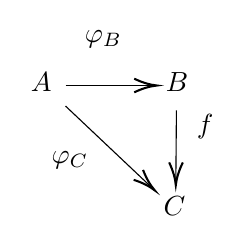
\begin{tikzpicture}[x=0.75pt,y=0.75pt,yscale=-1,xscale=1]
  %uncomment if require: \path (0,300); %set diagram left start at 0, and has height of 300


  % Text Node
  \draw (111,62.4) node [anchor=north west][inner sep=0.75pt]    {$A$};
  % Text Node
  \draw (176,62.4) node [anchor=north west][inner sep=0.75pt]    {$B$};
  % Text Node
  \draw (175,122.4) node [anchor=north west][inner sep=0.75pt]    {$C$};
  % Text Node
  \draw (137,42.4) node [anchor=north west][inner sep=0.75pt]    {$\varphi _{B}$};
  % Text Node
  \draw (121,100.4) node [anchor=north west][inner sep=0.75pt]    {$\varphi _{C}$};
  % Text Node
  \draw (191,82.4) node [anchor=north west][inner sep=0.75pt]    {$f$};
  % Connection
  \draw    (129,70) -- (171,70) ;
  \draw [shift={(173,70)}, rotate = 180] [color={rgb, 255:red, 0; green, 0; blue, 0 }  ][line width=0.75]    (10.93,-3.29) .. controls (6.95,-1.4) and (3.31,-0.3) .. (0,0) .. controls (3.31,0.3) and (6.95,1.4) .. (10.93,3.29)   ;
  % Connection
  \draw    (129,79.92) -- (170.55,119.18) ;
  \draw [shift={(172,120.55)}, rotate = 223.38] [color={rgb, 255:red, 0; green, 0; blue, 0 }  ][line width=0.75]    (10.93,-3.29) .. controls (6.95,-1.4) and (3.31,-0.3) .. (0,0) .. controls (3.31,0.3) and (6.95,1.4) .. (10.93,3.29)   ;
  % Connection
  \draw    (182.4,82) -- (182.12,116) ;
  \draw [shift={(182.1,118)}, rotate = 270.48] [color={rgb, 255:red, 0; green, 0; blue, 0 }  ][line width=0.75]    (10.93,-3.29) .. controls (6.95,-1.4) and (3.31,-0.3) .. (0,0) .. controls (3.31,0.3) and (6.95,1.4) .. (10.93,3.29)   ;

\end{tikzpicture}
\end{definition}

\begin {definition} \label{modulo}
Sea $A$ un anillo, se llama $A$-módulo a cualquier grupo abeliano $(M,+)$ de $(A,+)$ junto con una operación externa $A\times M \to M$ que cumpla que para todo $m,n \in M, a,b \in A$:
\begin{enumerate}
  \item $a(m+n) = am + an$
  \item $(a+b)m = am+bm$
  \item $(ab)m = a(bm)$
  \item $1_Am = m$.
\end{enumerate}
\end{definition}

\begin{example}
\begin{enumerate}
  \item Si $\mathbb K $ es un cuerpo, todo $\mathbb K$-espacio vectorial es un $\mathbb K$-módulo..
  \item Si $V$ es un $\mathbb K$-espacio vectorial de dimensión finita y $f:V\to V$ un endomorfismo, entonces $V$ es un $\mathbb K[x]$-módulo via la aplicación

  \begin{align*}
    {\mathbb K[x]\times V} & \to     V                                 \\
    {(p(x),v)}             & \mapsto p(f) = a_nf^{(n)}+\dots+a_1 f+a_0
  \end{align*}
  siendo $p(x) = a_nx^n+\dots+a_1x + a_0$ y $f^(k) = f\circ \overset{k)}{\dots} \circ f$.
  \item Toda $A$-álgebra $B$ de un anillo $A$ es un $A$-módulo. $B$ es un anillo luego $(B,+)$ es un grupo abeliano. Por ser $A$-álgebra, existe un homomorfismo $\varphi:A\to B$, y entonces podemos definir la operación externa de la definición \ref{modulo} como $A\times B \to B$ que hace corresponder $(a,b) \mapsto\varphi(a)b$.
\end{enumerate}
\end{example}

\begin{remark} \label{prop_adicional}
Atendiendo al último ejemplo resulta que dados dos anillos $A, B$, dar a $B$ estructura de $A$-álgebra es equivalente a darle estructura de $A$-módulo junto con la propiedad adicional de que
\[\forall b, b' \in B, \; \forall a \in  A \quad a \cdot_{\text{ext}} (bb') = (a\cdot_{\text{ext}} b) b'\]
\end{remark}

\begin{definition}
  Sea $B$ una $A$-álgebra mediante $f:A\to B$. Se dice que $B$ está finitamente generada si existen $b_1, \dots, b_r \in B$ tales que para todo $x \in B$ se cumpla

  \[x = \sum _{i_1, \dots, i_r} f(a_{i_1,\dots,i_r}) b_1^{i_1}\dots b_r^{i_r}\]
\end{definition}

\begin{remark}
Sea $B$ una $A$-álgebra, si utilizamos la caracterización de la observación \ref{prop_adicional}, entonces $B$ es finitamente generada si y solo si existen $b_1,\dots, b_r \in B$ tales que para todo $x \in B$ se escribe $x = \sum _{i_1, \dots, i_r} a_{i_1,\dots,i_r} b_1^{i_1}\dots b_r^{i_r}$.

En el caso particular en que $A\subset B$, entonces $B$ es una $A$-álgebra finitamente generada si y solo si $B = A[b_1, \dots, b_r]$ para ciertos $b_1,\dots, b_r \in B$, es decir, el menor anillo que contiene a $A$ y a los $b_i$.
\end{remark}
\begin{example}
\begin{enumerate}
    \item Si $A$ es un anillo, entonces $A\subset A[X_1, \dots, X_n]$ y el anillo de polinomios es una $A$-álgebra finitamente generada.
    \item Sean $A$ subanillo de $B$, con $B$ una $A$-álgebra finitamente generada por $\{b_1,\dots,b_r\}$. Se puede tomar el anillo de polinomios $A[X_1,\dots,X_r]$ y el homomorfismo evaluación en los $b_i$:
    \begin{align*}
        \operatorname{eval}_{b_1,\dots, b_r}:A[X_1,\dots,X_r] &\to B\\
        X_i &\mapsto b_i\\
        A \ni a &\mapsto a
    \end{align*}
    El homomorfismo $\operatorname{eval}_{b_1,\dots, b_r}$ es suprayectivo porque los elementos de $B$ son expresiones polinomiales en $b_1,\dots, b_r$. Aplicando el primer teorema de isomorfía tenemos
    \[\faktor{A[X_1,\dots,X_r}{\ker \operatorname{eval}_{b_1,\dots, b_r}} \cong B\]
    \item Más generalmente, si $B$ es una $A$-álgebra finitamente generada, también es una $f(A)$-álgebra finitamente generada y se puede repetir el ejemplo anterior con $f(A)$, que es subanillo de $B$.
\end{enumerate}

\end{example}

\section{Uso del lema de Zorn en álgebra conmutativa}

\begin{definition}
  Sea un conjunto parcialmente ordenado $(S,\leq)$. Una cadena $T \subset S$ es un subconjunto tal que para cualesquiera $x,y \in T$ se cumple $x\leq y$ o $ y \leq x$.
\end{definition}

\begin{lemma} \textbf{\emph{(de Zorn)}}
Sea un conjunto parcialmente ordenado $(S,\leq)$. Si toda cadena $T \subset S$ tiene una cota superior, entonces existe un elemento maximal en $S$.
\end{lemma}

\begin{proposition} \label{existe_maximal}
Todo anillo $A \neq 0$ tiene un ideal maximal
\end{proposition}
\begin{proof}
Consideramos el conjunto $\Sigma$ de los ideales propios de $A$, que no es vacío porque $0\in \Sigma$, y lo ordenamos con la inclusión. Sea $(\mathfrak a_i)_{i\in I}$ una cadena en $\Sigma$. Veamos que tiene una cota superior.
Consideramos $\mathfrak a ^* = \bigcup _{i\in I} \mathfrak a_i$, que es un ideal:
\begin{enumerate}
    \item Para todos $x, y \in  \mathfrak a^*$ existen $i, j \in I$ tales que $x\in \mathfrak a_i$ e $y \in \mathfrak a_j$. Como pertenecen a una cadena, podemos suponer que $\mathfrak a_i \subset \mathfrak a_j$ y por tanto $x, y \in \mathfrak a_j$, que es un ideal, luego $x - y \in  \mathfrak a_j \subset a^*$.
    \item Para todo $x\in \mathfrak a^*$ y todo $a \in A$, existe $i\in I$ tal que $x\in \mathfrak a_i$ y por tanto $xa \in \mathfrak a_i \subset \mathfrak a^*$.
\end{enumerate}
Además, es un ideal propio porque $1\not\in \mathfrak a_i$ para todo $i\in I$ luego no pertenece a la unión. Entonces $\mathfrak a^* \in \Sigma$ y está claro que es una cota superior de la cadena, que es arbitraria. Podemos aplicar el lema de Zorn y concluimos que $\Sigma$ tiene un elemento maximal, y por tanto $A$ tiene un ideal maximal.
\end{proof}

\begin{corollary}
Para todo ideal $\mathfrak a$ de un anillo $A$ existe un ideal maximal que lo contiene
\end{corollary}
\begin{proof}
Se aplica la proposición anteior al anillo $\faktor{A}{\mathfrak a}$ teniendo en cuenta que en el teorema de la correspondencia se conservar los ideales maximales.
\end{proof}

\begin{proposition}
Sea $A$ anillo, existe un ideal primo minimal\footnote{Un ideal primo que no contiene a ningún otro ideal primo.} $\mathfrak p$.
\end{proposition}
\begin{proof}
Sabemos que existe un ideal maximal $\mathfrak{p} \subset A$, y este es primo por ser maximal. Consideramos $\Sigma$ el conjunto de los ideales primos de $A$, que es no vacío porque $\mathfrak p \in \Sigma$, y lo ordenamos parcialmente con la inclusión tal que $\mathfrak p \leq \mathfrak p' \iff \mathfrak p \supset \mathfrak p'$ . Sea $\{\mathfrak{q}_{i}\}_{i \in I} \subset \Sigma$ una cadena y consideramos $\mathfrak{q}^{*}:=\bigcap_{i \in I} q_{i}$. Este es un ideal (la intersección siempre lo es) y $\mathfrak{q}^{*} \subset \mathfrak{q}_{i}$ para todo $i\in I$, por tanto es cota superior (para nuestro orden) de la cadena.

Veamos que $\mathfrak{q}^{*}$ es primo. Sean $a b \in \mathfrak{q}^{*},$ por ser así, $a b \in \mathfrak{q}_{i}$ para toda $i \in I .$ Si $a \in \mathfrak{q}_{i} \forall i \in I,$ entonces $a \in \mathfrak{q}^{*}$. Por otra parte, si existe $i_{0} \in I$ tal que $a \notin \mathfrak{q}_{i_{0}}$
$$
\begin{array}{l}
\text { entonces } b \in \mathfrak{q}_{j} \forall j \in I: \\
\qquad \text { si } \mathfrak{q}_{i_{0}} \subseteq \mathfrak{q}_{j}, \text { como } b \in \mathfrak{q}_{i_{0}}, \text { se tiene que } b \in \mathfrak{q}_{j} \mathrm{y},
\end{array}
$$

Así se tiene $\mathfrak q^* \in \Sigma$ y aplicando el lema de Zorn, existe un elemento maximal para el orden dado, equivalemente, minimal en sentido de la inclusión.
\end{proof}

\begin{corollary}
Sea $A$ anillo y $\mathfrak a$ ideal de $A$, existe un ideal primo minimal entre los que contienen a $\mathfrak a$.
\end{corollary}

\begin{definition}
Sea $A$ un anillo. Un elemento $x\in A$ se dice \emph{nilpotente} si existe un $n\in \mathbb N \setminus \{0\}$ tal que $x^n = 0$.
\end{definition}

\begin{definition}
Sea $A$ un anillo. El \emph{radical} de un ideal $\mathfrak a$ de $A$ se define como
\[\sqrt {\mathfrak a} = \{x\in A: \; \exists n>0 \text{ tal que } x^n \in \mathfrak a \} \]
\end{definition}

\begin{proposition}
Sea $A$ un anillo, entonces el conjunto $\mathfrak N_A$ de todos los elementos nilpotentes de $A$ es un ideal. Se le llama \emph{nilradical} de $A$.
\end{proposition}
\begin{proof}
\begin{enumerate}
    \item Si $x \in \mathfrak{N}_A$ y $a\in A$, existe $n>0$ tal que $x^n = 0$ y por tanto $(xa)^n = x^na^n = 0$.
    \item Si $x,y \in \mathfrak N_A$, existen $m, n>0$ tales que $x^n = y^m = 0$. Utilizando el binomio de Newton se tiene que $(x+y)^{n+m-1}$ es una suma de multiplos de productos de la forma $x^ry^s$ con $r+s = m+n-1$, y por tanto no se puede tener a la vez $r<n$ y $s<m$, de manera que cada uno de los sumandos es $0$ y $(x+y)^{n+m-1}=0$.
\end{enumerate}
\end{proof}

\begin{proposition}
El nilradical de un anillo $A$ verifica $\mathfrak N_A = \bigcap_{\mathfrak p \text{ primo}} \mathfrak p$.
\end{proposition}
\begin{proof}
Denotamos por $\mathfrak N$ a la intersección. Si $x\in \mathfrak N_A$ entonces existe $n>0$ con $x^n = 0$. El cero pertenece a todo ideal, en particular para todo $\mathfrak p$ primo $0= x^n = x x^{n-1} \in \mathfrak p$, lo que implica que $x \in \mathfrak p$ (porque o bien $x\in\mathfrak p $ o bien $x^{n-1}\in \mathfrak p$ y repetimos). Por tanto $x\in \mathfrak N$ y $\mathfrak N_A \subset \mathfrak N$.

Para ver el otro contenido, comprobamos que si $x_0 \not \in \mathfrak N_A$ entonces existe $\mathfrak p$ primo tal que $x\not \in \mathfrak p$. Sea $\Sigma = \{\mathfrak a : \; \text{ideal propio tal que } x_0^n \not \in \mathfrak a \text{ para todo } n>0 \}$, que es un conjunto no vació porque pertenece el $0$, ya que si $x_0$ no es nilpotente, ninguna de sus potencias es $0$, así que $x_0^n \not \in \{0\}$ para todo $n$. Argumentamos igual que en la proposición \ref{existe_maximal} y obtenemos un elemento maximal de $\mathfrak p^* \in \Sigma$.

Veamos que $\mathfrak p^*$ es primo, equivalentemente, que si $x, y \not \in \mathfrak p^*$, entonces $xy\not\in \mathfrak p^*$. Sean entonces $x,y \not \in \mathfrak p^*$, y consideramos $\mathfrak p^* + (x)$ y $\mathfrak p^* + (y)$ ideales que contienen a $\mathfrak p^*$ estrictamente. Como $\mathfrak  p^*$ es un elemento maximal de $\Sigma$, esos dos ideales no pueden pertenecer a $\Sigma$, así que por definición existen $m, n>0$ tales que $x_0^n\in \mathfrak p^* + (x)$ y $x_0^m \in \mathfrak p^* + (y)$. Entonces existen $p,q \in \mathfrak p^*$ tales que

\[x_0^{m+n} = x_0^n x_0^m = (p+x)(q+y) = \underset{\in \mathfrak p}{pq} + \underset{\in (xy)}{py} + \overset{\in (xy)}{qx} + \overset{\in (xy)}{xy} \in \mathfrak p^* + (xy) \]

Por tanto $\mathfrak p^*+(xy) \not \in \Sigma$, y como $\mathfrak p^* \in \Sigma $, entonces $xy \not \in \mathfrak p ^*$.
\end{proof}

\section{Extensión y contracción de ideales}

\begin{definition}
Sea $\phi:A\to B$ un homomorfismo de anillos y sea $\mathcal I(A), \mathcal I(B)$ los conjuntos de ideales de $A$ y $B$. Se define la \emph{extensión de ideales} como la aplicación
\begin{align*}
    e:\mathcal I(A) &\to \mathcal I(B) \\
    \mathfrak a &\mapsto \mathfrak a^e =\left \{\sum_{i=1}^m \phi(a_i)b_i \bigg\vert \; a_i \in \mathfrak a, b_i \in B, m\in \mathbb N \right \}
\end{align*}
y la \emph{contracción de ideales} como
\begin{align*}
    c:\mathcal I(B) &\to \mathcal I(A) \\
    \mathfrak{b} &\mapsto \phi^{-1}(\mathfrak b)
\end{align*}
\end{definition}

\begin{remark} \textbf{Propiedades de la extensión y la contracción}

\begin{enumerate}
    \item La contracción conserva ideales primos: si $\p$ es un ideal primo de $B$, entonces $\p^c$ es un ideal primo de $A$.
    \item El comportamiento de $e$ y $c$ respecto de las operaciones anteriores es el siguiente\begin{align*}
        (\af_1+\af_2)^e=(\af_1)^e+(\af_2)^e\hspace{15pt}& (\bfr_1+\bfr_2)^c\subseteq(\bfr_1)^c+(\bfr_2)^c\\
        (\af_1\cap\af_2)^e\subseteq(\af_1)^e\cap(\af_2)^e\hspace{15pt}&(\bfr_1\cap\bfr_2)^c=(\bfr_1)^c\cap(\bfr_2)^c\\
        (\af_1\af_2)^e=(\af_1)^e(\af_2)^e\hspace{15pt}& (\bfr_1\bfr_2)^c\subseteq(\bfr_1)^c(\bfr_2)^c
    \end{align*}
\end{enumerate}
\end{remark}

\section{Lenguaje geométrico en álgebra conmutativa}

\begin{definition}
Sea $K$ un cuerpo, se dice que es \emph{algebraicamente cerrado} si se cumple cualquiera de las condiciones equivalentes:
\begin{enumerate}
    \item Para todo $f\in K[x]\setminus\{0\}$ existe $a\in K$ tal que $f(a)=0$.
    \item Todo $f\in K[x]\setminus\{0\}$ se descompone en factores de primer grado, es decir, si $\deg f = n$, $f(x) =\lambda \prod_{i=1}^n (x-a_i)$ para ciertos $\lambda, a_1, \dots, a_n$.
    \item Toda extensión algebraica $L\vert K$ es trivial: $L = K$.
\end{enumerate}
\end{definition}

\begin{proposition}
Para todo cuerpo $K$ existe una extensión $L|K$ algebraicamente cerrada.
\end{proposition}
\begin{proof}
Ver teorema II.2.4 en \cite{gamboa}.
\end{proof}

\begin{example}
\begin{enumerate}
  \item $\mathbb{F}_p:=\Z/\langle p\rangle$, $p\in\Z$ primo
  \item $\mathbb{F}_{p^e}:=\mathbb{F}_p[x]/\langle f(x)\rangle$ donde $f(x)$ es irreducible en $\mathbb{F}_p$ y de grado $e$. Se verifica que $\mathbb{F}_{p^{e}}\subset\mathbb{F}_{p^{e'}}$ si, y sólo si, $e|e'$.
\end{enumerate}
\end{example}

\begin{definition}
Si $K$ es un cuerpo y $S\subset K[X_1, \dots, X_n]$, entonces se dice que
\[Z_{\mathbb A^n_K} = \{a \in \mathbb A^n_K \big \vert \; f(a) = 0 \text{ para cada } f\in S \} \]
es un \emph{conjunto algebraico} en $\mathbb A^n_K$.
\end{definition}

El estudio de los conjuntos de ceros de polinomios está íntimamente relacionado con el estudio de ideales porque $Z ( S) = Z ( \gen{S} )$. Efectivamente, si $a\in Z(\gen S)$, como $S \subset \gen S$, entonces en particular $a$ anula a todo polinomio de $S$, luego $Z ( S) \supset Z ( \gen{S} )$. Recíprocamente, sea $a'\in Z(S)$ y $g \in \gen S$ entonces existen $f_i\in S, g_i \in K[X_1,\dots, X_n]$ para $i = 1,\dots, m$ tales que $g(a') = \sum_{i=1}^m f_i(a')g_i(a') = 0$, así que $Z ( S) \subset Z ( \gen{S} )$.

\begin{example}
Sea un cuerpo $K$ algebraicamente cerrado y estudiemos los conjuntos algebraicos de $K[X]$ en $\mathbb A^1_K$. Solo hay tres tipos:
\begin{enumerate}
    \item $ Z(0) = \mathbb A^1_K$ porque el $0$ se anula en todas partes.
    \item $Z(K[X]) = \varnothing$ porque hay polinomios constantes no nulos.
    \item Si $g(x) = \gen {\prod_{i=1}^n (x - a_i)}$, entonces $ Z(g) = {a_1,\dots, a_n}$ porque un $f$ se anula en todos los $a_i$ si y solo si es múltiplo de $\prod_{i=1}^n (x-a_i)$.
\end{enumerate}
\end{example}

Si $K$ es un cuerpo, para todo $f\in K[x]$ se pueden encontrar $f_1,\dots, f_r$ sin factores irreducibles en $K[x]$ múltiples tales que $f = f_1 f_2^2 \dots f_r^r$. En particular, $f_{\operatorname{red}} = f_1f_2 \dots f_r$ es un polinomio con mismos ceros que $f$ pero de multiplicidad $1$ \footnote{Ver apéndice.}. Esto es útil, porque como $K[X]$ es un DIP, todo ideal es de la forma $\mathfrak a = f K[x] $. Dicho $f$ puede ser en principio más complejo de lo que es necesario, por ejemplo, para definir el conjunto algebraico $\{x \in \mathbb R \vert \; x^2 = 0 \}$ podemos usar, en vez de $x^2$, el polinomio $x$.

\begin{lemma} \label{lemita}
Sea $K$ un cuerpo, si $\mathfrak{a}\subset \mathfrak b$ son ideales de $K[X_1,\dots, X_n]$, entonces $Z(\mathfrak{a}) \supsetZ (\mathfrak b)$.
\end{lemma}

\begin{proposition}
Sea $K$ un cuerpo y $A = K[X_1,\dots , X_n]$
\begin{enumerate}
    \item Si $\{\mathfrak a_i\}_{i\in I}$ una familia arbitraria de ideales de $A$, entonces $Z(\sum_i \mathfrak a_i) = \bigcap_i Z(\mathfrak a_i)$.
    \item Si $\{\mathfrak b_j\}_{j = 1}^m$ una familia finita de ideales de $K[X_1,\dots , X_n]$, entonces $\bigcup_{j=1}^m Z(\mathfrak b_j) = Z(\mathfrak b_1 \dots \mathfrak b_m)$.
\end{enumerate}
\end{proposition}
\begin{proof}
Por orden

1. Sea $a\in Z(\sum_i \mathfrak a_i)$. Cualquier $f_i \in \mathfrak a_i$ es en particular un elemento de $\sum_i \mathfrak a_i$ así que $f_i(a)  = 0$. Como $i$ es arbitrario y $f_i$ también, entonces $a \in \bigcap_i Z(\mathfrak a_i)$.

 Denotando $\af^*=\underset{i\in I}{\Sigma}\af_i$, dado $f\in\af^*$ tenemos que $f=f_{i_1}+\cdots+f_{i_r}$ para ciertos $\{i_1,\dots,i_r\}\subseteq I$ y donde $f_{i_j}\in\af_{i_j}$. Si tomamos $a\in\bigcap Z(\af_i)$, entonces $f(a)=f_{i_1}(a)+\cdots+f_{i_r}(a)=0$, es decir, $a\in Z(\af^*)$.



2. Comprobamos el doble contenido. Primero, como $\mathfrak a \cdot \mathfrak b \subset ( \mathfrak a \cap \mathfrak b )$ y este está contenido en ambos $\mathfrak a$ y $\mathfrak b$, entonces por el lema \ref{lemita} $\zeros {\mathfrak a}, \zeros{\mathfrak b}\subset \zeros{\mathfrak a \cdot \mathfrak b} $, y así su unión también está contenida.

El otro contenido lo hacemos por contrarrecíproco.  Si $a\not\in \zeros{\mathfrak a}\cup \zeros{\mathfrak b}$, entonce es que $a\not\in \zeros{ \mathfrak a}$ y $a\not\in \zeros{ \mathfrak b}$. Existen $f\in \mathfrak a$ y $g\in \mathfrak b$ tales que $f(a)\neq 0$ y $g(a) \neq 0$, por tanto $fg(a) = f(a)g(a) \neq 0$, y entonces $a\not\in \zeros{\mathfrak a\cdot \mathfrak b}$.

\end{proof}

De acuerdo a lo que hemos visto, los conjuntos algebraicos en $\mathbb A^n_K$ son una colección $\mathcal A$ de subconjuntos que cumplen:
\begin{enumerate}
    \item $\varnothing, \mathbb A^n_K \in \mathcal A$,
    \item la intersección arbitraria de conjuntos de $\mathcal A$ pertenece a $\mathcal A$,
    \item la unión finita de conjuntos de $\mathcal A$ pertenece a $\mathcal A$.
\end{enumerate}
Estos son los tres axiomas que debe cumplir una familia de conjuntos para ser los cerrados de una \emph{topología}.

\begin{example} $\A_K^1$ es un espacio topológico con la topología de los complementarios finitos.
\end{example}


\begin{theorem} \textbf{\emph{(de la base de Hilbert)}}
Si $A$ es un anillo tal que todo ideal de $A$ está finitamente generado, entonces $A[X]$ también cumple esa propiedad.
\end{theorem}
\begin{proof}
Sea $\mathfrak{I} \subset A[x]$ un ideal, y formamos el conjunto de los coeficientes principales de polinomios en $\mathfrak{I}$.
$$
\mathfrak a = \{c \in A\setminus\{0\}\vert \; \exists r \in \mathbb N \text{ con } cx^r+ \text{tmg} \in \mathfrak i\}\cup \{0\} \footnote{Aquí tmg significa términos de menor grado. Expresamos así el polinomio porque no será necesario prestar atención al resto.}
$$

Comprobamos que $\mathfrak a$ es un ideal.

\begin{enumerate}
    \item Sean $c,d \in \mathfrak a$. Si $c=d$ entonces $c-d =0\in \mathfrak a$. Si $c\neq d$, entonces existen $r,s$ tales que $f = cx^r+\text{tmg}, g = dx^s+\text{tmg} \in \mathfrak I$. Entonces por ser $\mathfrak{I}$ un ideal tenemos que
    \[\mathfrak{I} \ni f-x^{r-s}g = (c-d)x^{r}+\text{tmg}\]
    con lo que $c-d \in \mathfrak a$ también.
    \item Sean $c\in \mathfrak a$ y $\lambda \in A$. Si $\lambda = 0$ es trivial. Si no, existe $f\in \mathfrak{I}$ con $c$ de coeficiente principal, y $\lambda f \in \mathfrak{I}$ tiene a $\lambda c$ de coeficiente principal, luego $\lambda c \in \mathfrak a$.
\end{enumerate}

Por hipótesis, $\mathfrak a$ está finitamente generado $\mathfrak a = \gen{c_1, \dots, c_s}$. Para cada $i=1,\dots, s$ existe un $f_i\in \mathfrak{I}$ con $c_i$ como coeficiente principal. Sea $\delta = \max_{1\leq i \leq s} \deg f_i$, y para cada $\gamma \leq \delta$ definimos

\[ \mathfrak{a}_\gamma = \{d \in A\setminus\{0\} \vert \; \exists f \in \mathfrak{I} \text{ con } \deg f = \gamma \text{ y con } d \text{ como coeficiente principal}\}\cup \{0\}\]

que también es un ideal de $A$:

\begin{enumerate}
    \item Sean $c,d \in \mathfrak{a}_\gamma$. Si $c=d$ entonces $c-d =0\in \mathfrak a$. Si $c\neq d$, entonces existen $f, g\in \mathfrak{I}$ de grado $\gamma$ con coeficientes principales $c, d$ respectivamente, entonces $f-g\in \mathfrak{I}$ es de grado $\gamma$ y tiene a $c-d$ por coeficiente principal.
    \item Si $c\in \mathfrak a$ y $\lambda \in A$. Si $\lambda = 0$ es trivial. Si no, existe $f\in \mathfrak{I}$ de grado $\gamma$ con $c$ de coeficiente principal, y $\lambda f \in \mathfrak{I}$ es de grado $\gamma$ y tiene a $\lambda c$ de coeficiente principal.
\end{enumerate}

De nuevo, por hipótesis, $\mathfrak{a}_\gamma$ es finitamente generado, así que $\mathfrak{a}_\gamma = \gen{d_{\gamma_1},\dots, d_{\gamma_m} }$, y para cada $j=1, \dots,m_\gamma$ existe un polinomio $g_{\gamma_j}\in \mathfrak{I}$ que tiene a $d_{\gamma_j}$ por coeficiente principal.

Vamos a comprobar que $\mathfrak{I} = \mathfrak{H}$ donde

\[\mathfrak{H}=\gen{\{f_1,\dots,f_s\} \cup \{g_{\gamma_j}\}_{\substack{1\leq \gamma \leq \delta\\ 1\leq j\leq m_\gamma}}} \subset \mathfrak{I}\]


El contenido $\supset$ se tiene por construcción. Para el otro, sea $F \in \mathfrak{I} \setminus \{0\}$ (si $\mathfrak{I} = \{0\}$, es trivial) y sea $\mu = \deg F$. Distinguimos dos casos.

\paragraph{Caso 1} Supongamos $\mu \geq \delta$, en caso contrario pasamos al caso 2. Sea $b\in \mathfrak a$ el coeficiente principal de $F$, entonces $b = \sum_{i=1}^s \lambda_ic_i$ para ciertos $\lambda_i\in A$.  Resulta entonces que

\[F_1 = F - \underset{\in \mathfrak{H}}{\underbrace{\sum_{i=1}^s \lambda_i x^{\mu-r_i} f_i}}\in \mathfrak{I}, \qquad r_i = \deg f_i  \]

es un polinomio de grado $<\mu$ por construcción. Además basta demostrar que $F_1 \in \mathfrak{H}$ para que $F\in \mathfrak{H} \subset \mathfrak{I}$.

Si $\mu_1 = \deg F_1 \geq \delta$, repetimos lo anterior para $F_1$ y obtenemos otro polinomio $F_2\in \mathfrak{I}$ de grado estrictamente menor que $\mu_1$. Se cumple entonces que $F = \text{(polinomio en }\mathfrak H + F_2$. Continuamos repitiendo hasta que obtenemos $F^*\in \mathfrak{I}$ de grado $\nu$ estrictamente menor que $\delta$.  Entonces
\begin{equation}\label{algoenJ}
    F =  \text{(polinomio en $\mathfrak H$)} + F^*
\end{equation}
y basta ver que $F^*$ está en $\mathfrak H$ para que $F\in \mathfrak H \subset \mathfrak I$. Pasamos al caso 2.

\paragraph{Caso 2} Como $\nu < \delta $, el coeficiente principal de $F^*$, $u$, está en $\mathfrak{a}_\nu$, o bien $F^*=0$ en cuyo caso hemos terminado por (\ref{algoenJ}). Como ese ideal está finitamente generado, tenemos $u = \sum_{j=1}^{m_\nu} t_j d_{\nu_j}$ para ciertos $t_j\in A$. Por definición de $\mathfrak {a}_\nu$, existen $g_{\nu_j}(x) \in \mathfrak H$ con $d_{\nu_j}$ como coeficiente principal para cada $j = 1, \dots, m_\nu$. Podemos imitar el caso 1 y formar

\[F^{*}_1 = F^* - \underset{\in \mathfrak{H}}{\underbrace{\sum_{j=1}^{m_\nu} t_j g_{\nu_j}}} \]

que por construcción es un polinomio de grado menor que $\nu$. Basta ver que $F^{*}_1 \in \mathfrak{H}$ para que $F^*\in \mathfrak{H}$. Podemos repetir este paso para $F^{*}_1$ y obtendremos otro polinomio $F^*_2\in \mathfrak I$, de manera que $F^*_1\in \mathfrak{H}$ si $F^*_2 \in \mathfrak H$. Como los grados de cada uno de los polinomios que obtenemos son cada vez menores, necesariamente en algún momento obtendremos un polinomio $F^{**} = 0 \in \mathfrak H$ y hemos terminado.


\end{proof}

\begin{corollary}
Si $A$ es tal que todo ideal está finitamente generado, entonces $A[X_1,\dots, X_n]$ también cumple es propiedad.
\end{corollary}

\begin{lemma} Sea $K$ un cuerpo y $f\in K[x]$. Se verifica que$$\sqrt{\langle f(x)\rangle}=\langle f_{\text{red}}(x)\rangle.$$
\end{lemma}
Demostración. Denotemos$$f(x):=f_1(x)f_2(x)^2\cdots f_r(x)^r$$donde $f_i$ es libre de cuadrados y $\text{mcd}(f_i,f_j)=1$ para cada par $i\neq j$. Si $g(x)\in K[x]$ es tal que existe $\nu\in\N$ de forma que $g(x)^\nu\in\lambda(x)f(x)$ para cierto $\lambda(x)\in K[x]$, entonces $f_i(x)|g(x)$. Más aún, por las propiedades de los $f_i$ se verifica que $\prod f_i(x)|g(x)$; es decir, $f_\text{red}(x)|g(x)$.

\begin{theorem} \textbf{\emph{(Nullstellensatz)}}
Sea $K$ un cuerpo algebraicamente cerrado y $\mathfrak a$ un ideal de $K[X_1,\dots,X_n]$, entonces

\[\mathfrak I (\zeros{\mathfrak a}) = \{ f\big \vert \; f(a) = 0 \text{ para todo } a \in\zeros{\mathfrak a} \} = \sqrt{\mathfrak a}\]
\end{theorem}

\begin{corollary}
 El mayor ideal $\bfr$ de $K[x_1,\dots,x_n]$ tal que $Z_K(\bfr)=Z_K(\af)$, para un $\af$ dado, es $\mathfrak{I}Z_K(\af)$.
\end{corollary}

\end{document}
